\chapter{Discrete Circuitry Design}
This chapter contains the discrete circuit which has been briefly reviewed in section \ref{section:SF}.
We built this circuit to apply the constant-current constant-voltage ($V_{DS}$) method to our nanowire device.

\section{Transforming the design from p-type measuring into n-type measuring}
In \cite{SF1}, the circuit is for p-type ISFET device (Fig.\ref{fig:SF_schematic_old}).
Our nanowire device is n-type.
Hence we transformed the circuit into the one in Fig.\ref{fig:SF_schematic}.
\begin{figure}[!htbp]
    \centering
    \includegraphics[width=0.8\textwidth] {../images/chapter4/SFdiscrete_old.png}
    \caption{The schematic of read-out circuit from \cite{SF1}. The ISFET is a p-type device. It is controlled by the current source $I_b$ whose sub-circuit is shown at right.}
    \label{fig:SF_schematic_old}
\end{figure}
\begin{figure}[!htbp]
    \centering
    \includegraphics[width=0.8\textwidth] {../images/chapter4/SFdiscrete_schematic.png}
    \caption{Our circuit schematic transformed from Fig.\ref{fig:SF_schematic_old}. The device under test (DUT) is a n-type device. It is controlled by the current source $I_b$ whose sub-circuit is shown at right.}
    \label{fig:SF_schematic}
\end{figure}


\section{Circuit Description}
The circuit is divided into two sections: the constant-voltage circuit and the constant-current source (Ib).

\subsection*{The constant-voltage circuit}
The constant-voltage circuit section has a source follower structure.
The input of the circuit is at the floating gate ($G$) of the device under test (DUT), where the output is at its source ($S$).

The $I_D$ of DUT is controlled by Ib.
Because The leakage current flowing into the negative input of OP2 is less than 0.1nA, the $I_D$ of the transistor should always be same as the current provided by Ib.

The $V_{DS}$ of DUT is always equal to the potential difference ($I_0 \times R_0$) across the resistor $R_0$.
This is achieved by two OP-based, unity-gain buffer.
They connected serially with $R_b$ and cause the voltage at the drain ($D$) to follow the voltage at the source ($S$).


\subsection*{The  constant-current source (Ib)}
The Ib circuit is in fact a current scaling down circuit.
By concerning the OP as ideal, the node $OP+$ has the same voltage as $OP-$.
This equalizes the potential difference between two resistors whose resistance are different by $N$-fold.
As a result, the currents $I_b$ and $I_s$ are also different by $N$-fold.
$I_b = I_s / N$.

The capacitor is for filtering. It filters the high frequency noise out to create a stable output current.


\section{Discrete Element}
We use tlc2264 made by Texas Instrument (TI) as our OP.
This OP requires a supply voltage of $\pm 5v$ and can perform rail-to-rail output operation.
Its open-loop gain (Large-signal differential voltage amplification rate) is 170 for the output load greater than 50k.

\begin{figure}[tb!hp]
    \centering
    \includegraphics[width=0.3\textwidth]{images/chapter4/LM334.png}
    \caption{LM334: The discrete element we use for current source Is. It has three terminals: $R$, $V_+$, $V_-$. The output current ($I_s$) flows from $V_+$ to $V_-$. The resistor $R_{SET}$ connected to $V_-$ and $R$ is for adjusting the output current.}
    \label{fig:lm334}
\end{figure}

\emph{For the current source Is and I0, we use lm334 (Fig.\ref{fig:lm334}) made by National Semiconductor.
It is a 3-terminal adjustable current sources with a wide dynamic cross voltage range of 1v to 40v (the cross voltage $V_{+} - V_{-}$ in Fig.\ref{fig:lm334}), and current accuracy of $\pm 3\%$.
In our experiment, the current $I_s$ is fixed at $1\mu A$ with an output impedance of $1.2G\Omega$.}


\section{Circuit Performance and Conclusion}
We examined the performance of our circuit by plotting its $I_D$-$V_G$ curve.
The $I_0$, $R_0$ and $V_G$ were kept constant.
We swept $I_D$ by changing the $N$ value with a variable resistor.
$N$ ranges from 1 to 1000.
And $I_b$ should range from $1\mu A$ to $1n A$.

We measured the output voltage at $S$ and subtracted this value from $V_G$ to get the corresponding $V_{GS}$.
These two values gave the $I_D$-$V_{GS}$ curve in Fig.\ref{fig:SF_result}.
We compare this curve with the curve obtained by directly sweeping $V_G$ and measuring $I_D$ with Source Meter (Keithley 2602).

\begin{figure}[!htb]
   \centering
   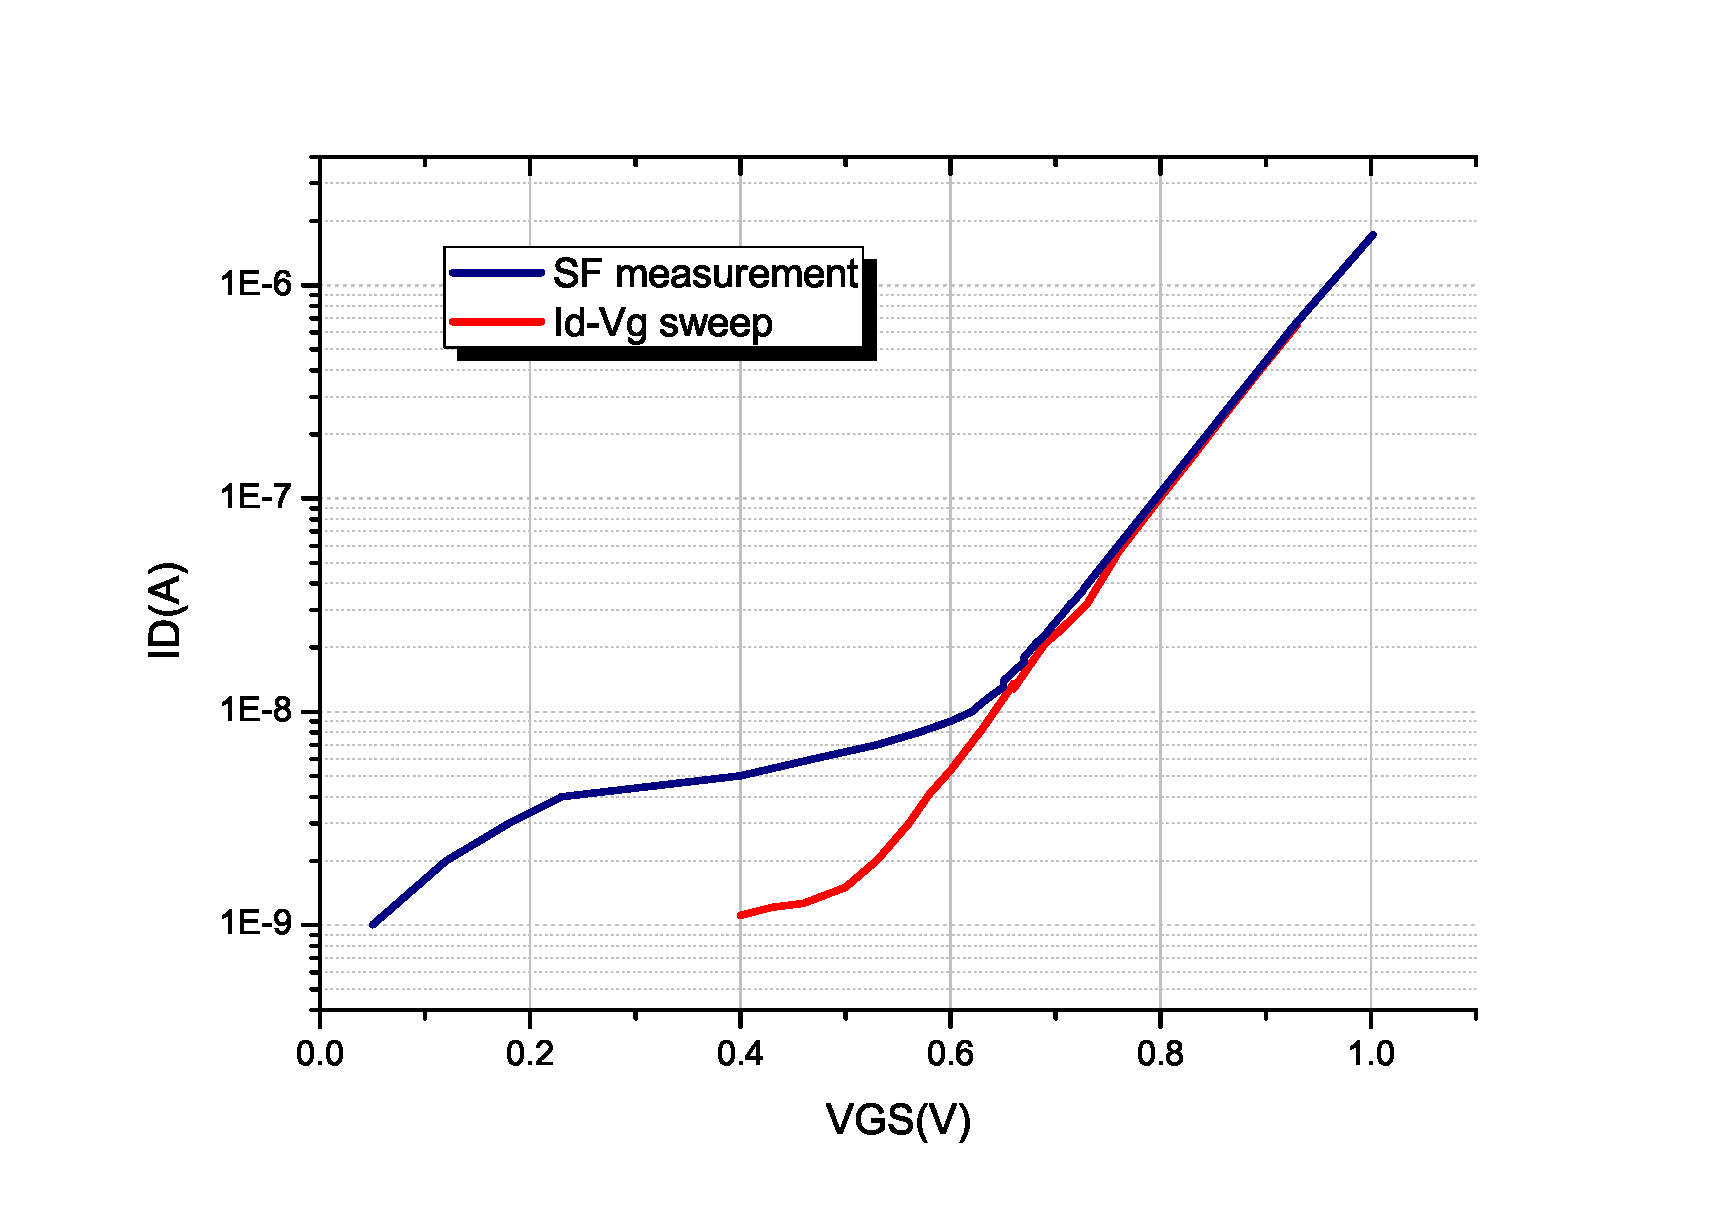
\includegraphics[width=1\textwidth]{images/chapter4/SF.eps}
   \caption{The measuremet result (``SF\_measurement'') compares with the direct $I_D$-$V_G$ sweep (``Id-Vg sweep'').}
   \label{fig:SF_result}
\end{figure}

The result shows that when $I_D$ is larger than $10n A$, the circuit is functional.
Two curves are same as each other.

The circuit fails when $I_D$ is smaller than $10n A$.
This is related to the impedance matching between the constant-voltage circuit and the Ib circuit, which we have discussed in section.\ref{section:SF}.

The output impedance of the Ib circuit is:
\begin{equation} \label{eq:rcs2_again}
    N\times R_s
\end{equation}
$R_s$ is the output impedance of the current source Is which equals to $1.2G\Omega$.
And the current input impedance at the $S$ of the constant-voltage circuit is:
\begin{equation} \label{eq:rsf2_again}
    \frac{1}{g_m}
\end{equation}

We plot the $I_b$-Impedance relationship in Fig.\ref{fig:SF_imp}.

\begin{figure}[!htb]
   \centering
   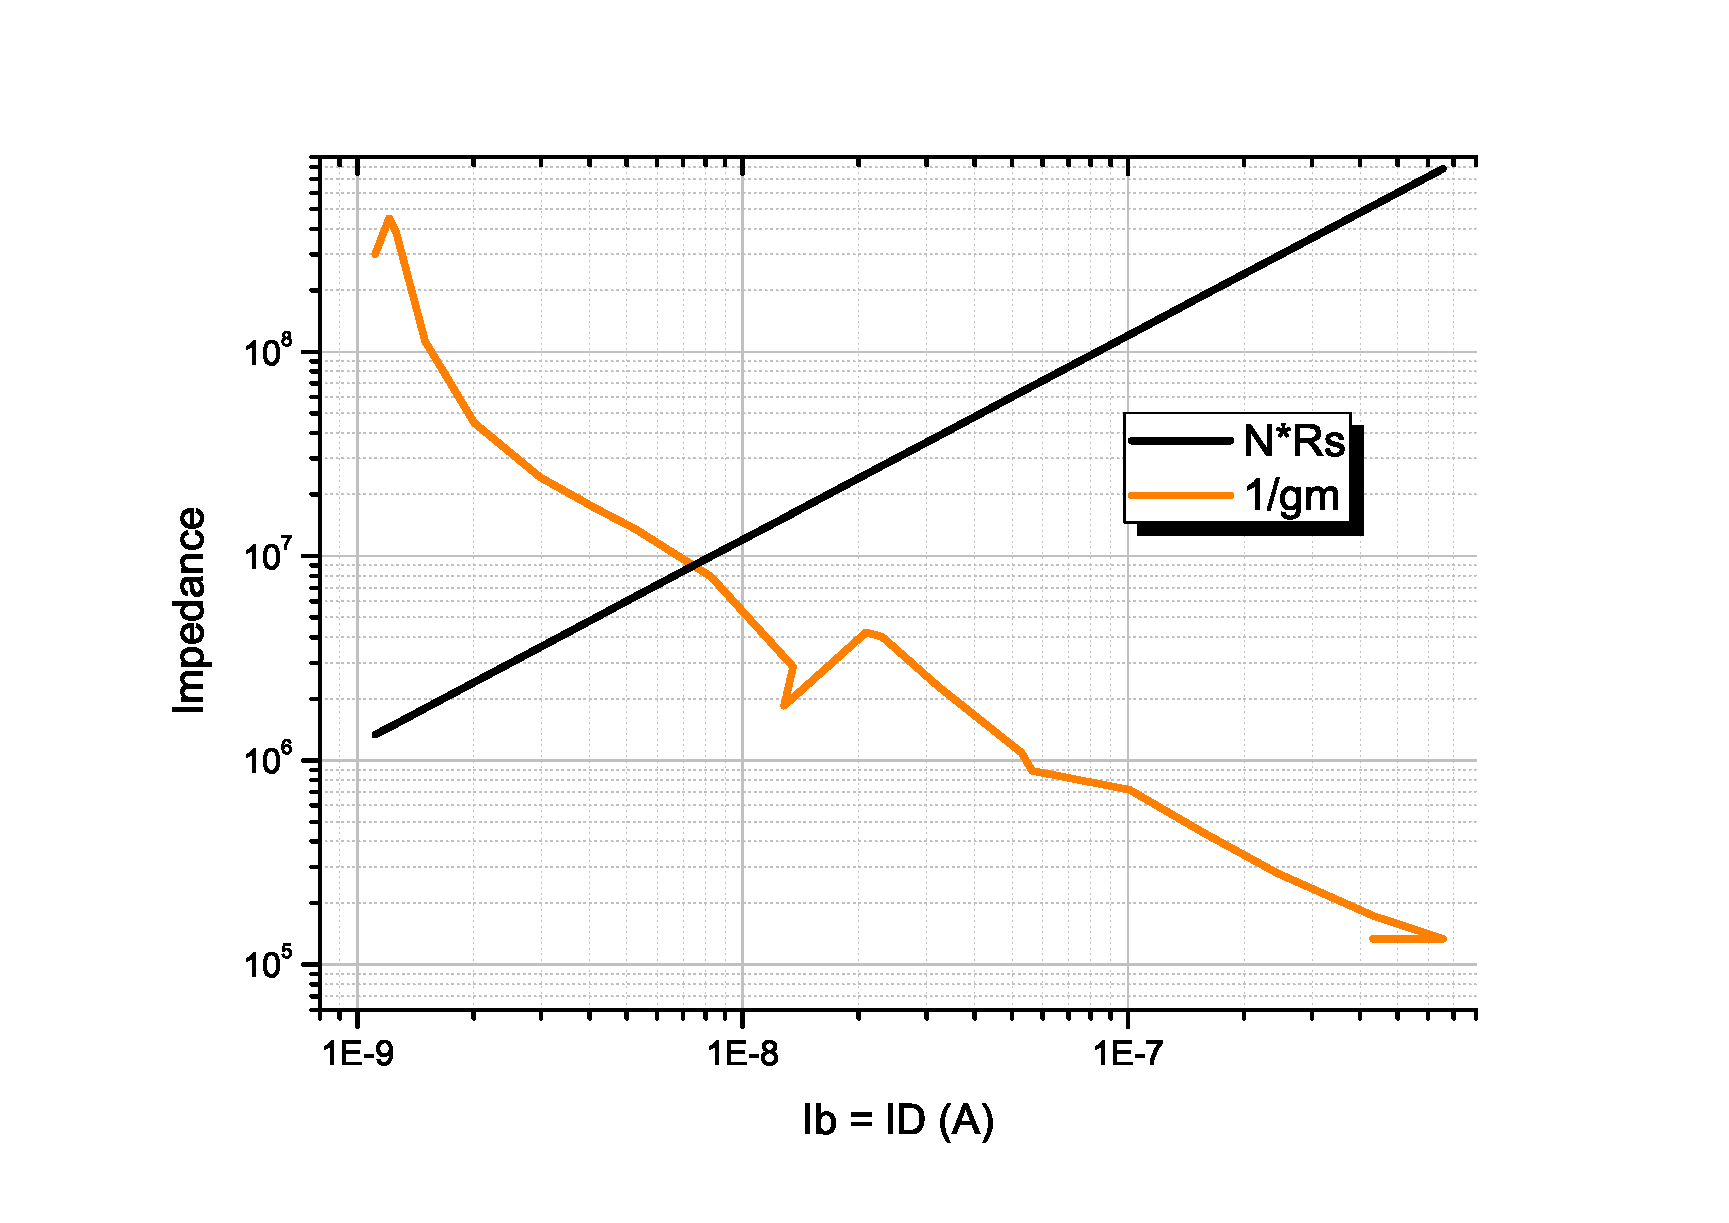
\includegraphics[width=1\textwidth]{../images/chapter4/SF_impedance.eps}
   \caption{Input impedance of transistor (``1/gm'') and output impedance of Ib circuit (``N * Rs''). The former is found by the derivative of $I_D$ of $V_{Gs}$. The latter is obtained by Eq.\ref{eq:rcs2_again}.}
   \label{fig:SF_imp}
\end{figure}


It shows that the output impedance of Ib is close to the input impedance of transistor when current is $10n A$ (N = 100).
The impedance is unmatched.

Overall, the constant-current constant-voltage method is feasible.
What one needs to notice when applying the this method is the impedance matching.
In the source follower structure, its current input impedance varies with the bias current.
It affects the dynamic range and needs more design concern.


